\section{Messungen und Auswertung}

	\subsection{Welche Netzform hat das 400-V-Drehstromnetz?}
		\begin{itemize}
			\item Bestimmen Sie durch eine Messung mit einem „Ohmmeter“ und mit einer Strom-Spannungsmessung  $(I\ <\ 100\ mA, R\ = 100\ \Omega)$ die Netzform des im Labortisches eingebauten 400V-Drehstromnetzes. Erläutern Sie Ihre Beobachtungen! 
			
			Mit einem Ohmmeter wurde ein Innenwiderstand von $O \Omega$ gemessen. Allerdings reicht die Messspannung des Ohmmeters nicht aus, um den Innenwiderstand $R_{NPE}$ zwischen N und PE zu erfassen. Dies kann durch die Verwendung einer Spannungsfehlerschaltung erreicht werden, bei der die Spannung mithilfe einer externen Quelle entsprechend angepasst werden kann.
			\newline
			\begin{align*}
				R_{NPE} &= \frac{U_{M}}{I_{M}}\\
				R_{NPE} &= \frac{50\ mV}{100\ mA}\\
				R_{NPE} &= 0,5 \Omega
			\end{align*}
			Wenn ein Innenwiderstand gemessen wurde, lässt dies darauf schließen, dass es sich um ein \textbf{TN-C-S-Netz} handelt. In diesem Netztyp sind der Neutralleiter und der Schutzleiter (PE) miteinander verbunden, was den Innenwiderstand erklärt.
		\end{itemize}
		
		
	\subsection{Fehlerstromschutzschalter zum Personenschutz}
		\begin{enumerate}[label=\alph*)]
			\item Ermitteln Sie den tatsächlichen Auslösestrom des FI-Schutzschalters durch Mittelwertbildung aus drei Messungen, benutzen Sie dazu Multimeter und den FI-Tester aus Bild 9. Nutzen Sie dazu die Min/Max-Funktion des Multimeters. Stellen Sie das Potentiometer auf einen großen Wert ein und verkleinern Sie dann langsam den Widerstandswert. Der Auslösestrom kann dann am Multimeter abgelesen werden.
			\begin{center}
				\begin{table}[h]
					\begin{tabular}{r l}
						\hline
						Anzahl & \( I\ in\ mA \) \\
						\hline
						1 & \( 20,75 \) \\
						2 & \( 20,60 \) \\
						3 & \( 20,00 \) \\
						\hline
						Mittelwert & \( 20,39\ mA \) \\
						\hline
					\end{tabular}
					\caption{Messwerte - Auslösestrom eines FI-Schutzschalters}
				\end{table}
			\end{center}
			
			
			\item Bestimmen Sie die Abschaltzeit bei Nennfehlerstrom des FI-Schutzschalters durch Mittelwertbildung aus drei Messungen, benutzen Sie dazu Multimeter, FI-Tester, Oszilloskop und Trennteiler. Ein Oszillogramm ist für die Ausarbeitung aufzubereiten! 
			3
			\begin{center}
				\begin{table}[h]
					\begin{tabular}{r l}
						\hline
						Anzahl & \( t\ in\ ms \) \\
						\hline
						1 & \( 27,77 \) \\
						2 & \( 28,99 \) \\
						3 & \( 25,89 \) \\
						\hline
						Mittelwert & \( 27,55\ ms \) \\
						\hline
					\end{tabular}
					\caption{Messwerte - Abschaltzeit eines FI-Schutzschalters}
				\end{table}
			\end{center}
			
		\end{enumerate}
 	
 	\subsection{Symmetrische Drehstromlast ohne/mit Kompensation}
	 	\begin{enumerate}[label=\alph*)]
	 		\item Bestimmen Sie die komplexen Effektivwerte der Spannungen $\underline{U}_{1N}$, $\underline{U}_{2N}$, $\underline{U}_{3N}$ und $\underline{U}_{NK}$ und der Ströme $\underline{I}_{1}$, $\underline{I}_{2}$, $\underline{I}_{3}$ und $\underline{I}_{K}$ bei angeschlossener symmetrischer Drehstromlast nach Bild 12. Skizzieren Sie die Messschaltung und verwenden Sie zur Messung Oszilloskop, Trennteiler und Stromwandler. Das Oszillogramm von $\underline{u}_{1}$ mit $\underline{i}_{1}$ ist mit in die Ausarbeitung zu übernehmen und aufzuarbeiten.
	 		 		
	 		\begin{center}
	 			\begin{table}[h]
	 				\begin{tabular}{r c c r c c}
	 					\hline
	 					Art & \( U_{eff}\ in\ V \) & \( Phase\ \varphi\ in\ ^\circ\ \ \)  & Art & \( I_{eff}\ in\ mA \) & \( Phase\ in\ ^\circ\ \ \) \\
	 					\hline
	 					$U_{1N}$ & \( 232 \) & \( 0 \) &
	 					$I_{1}$	 & \( 960 \) & \( -70 \) \\
	 					$U_{2N}$ & \( 234 \) & \( 240 \) &
	 					$I_{2}$	 & \( 900 \) & \( 170 \) \\
	 					$U_{3N}$ & \( 233 \) & \( 120 \) &
	 					$I_{3}$	 & \( 920 \) & \( 50 \) \\
	 					$U_{KN}$ & \( 0   \) & \( 0 \) &
	 					$I_{N}$	 & \( 0   \) & \( 0 \) \\
	 					\hline
	 				\end{tabular}
	 				\caption{Messwerte - Komplexen Effektivwerte der Spannungen und Ströme}
	 			\end{table}
	 		\end{center}
	 		
 			\begin{figure}[h!]
 				\centering
 					\begin{subfigure}[b]{0.5\textwidth}
 						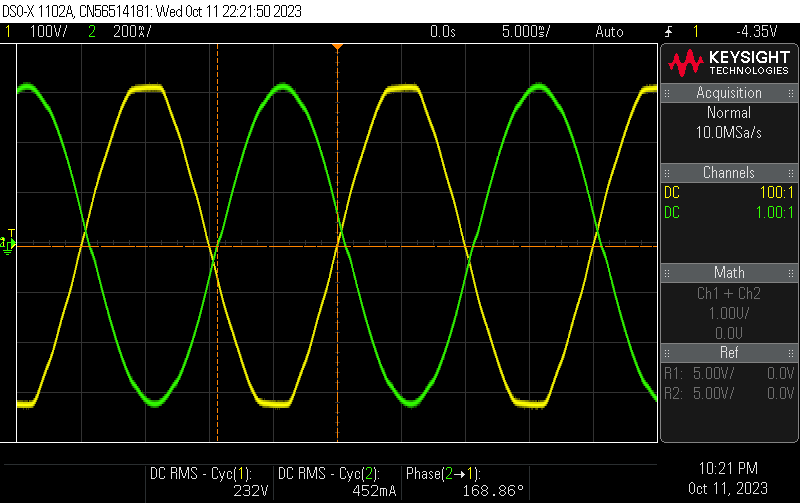
\includegraphics
 						[width=\textwidth]{img/img3.3.1.png}
 					\end{subfigure}\hfil
 				\caption{Oszillogramm von $u_{1}$ mit $i_{1}$ - Symmetrische Drehstromlast ohne Kompensation}\label{img3.3.1}
	 		\end{figure}
	 		
	 		\begin{figure}[h!]
	 			\centering
	 			\begin{subfigure}[b]{0.5\textwidth}
	 				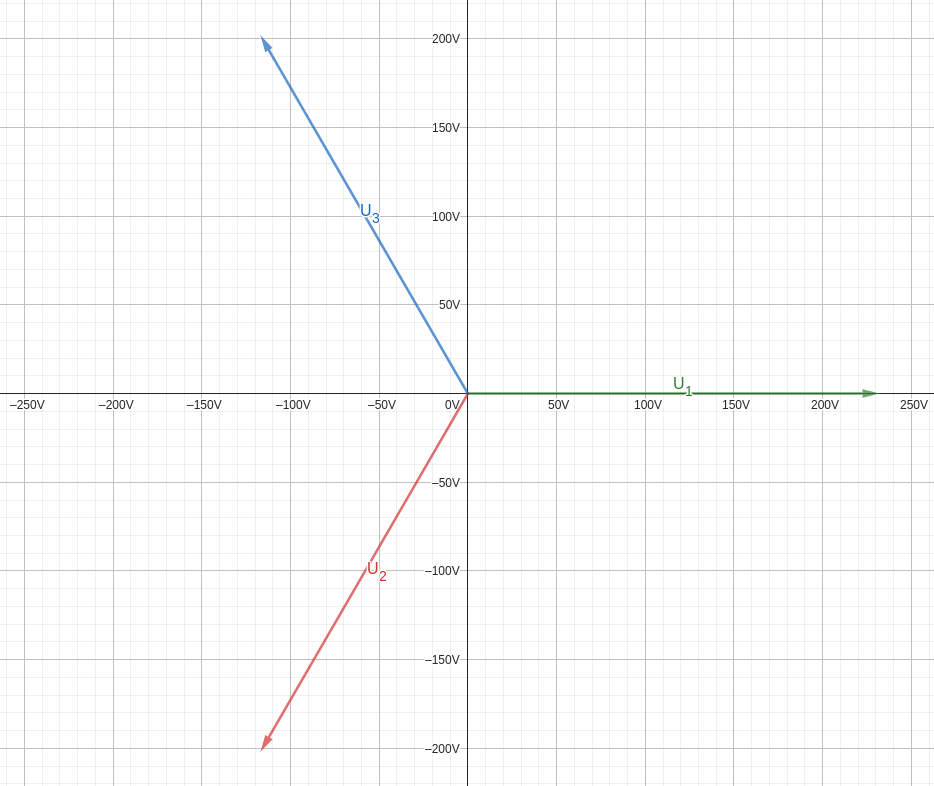
\includegraphics
	 				[width=\textwidth]{img/img3.3.2.png}
	 			\end{subfigure}\hfil
	 			\caption{Skizze der Spannungen - Symmetrische Drehstromlast ohne Kompensation}\label{img3.3.2}
	 		\end{figure}
	 			 		
	 		\begin{figure}[h!]
	 			\centering
	 			\begin{subfigure}[b]{0.5\textwidth}
	 				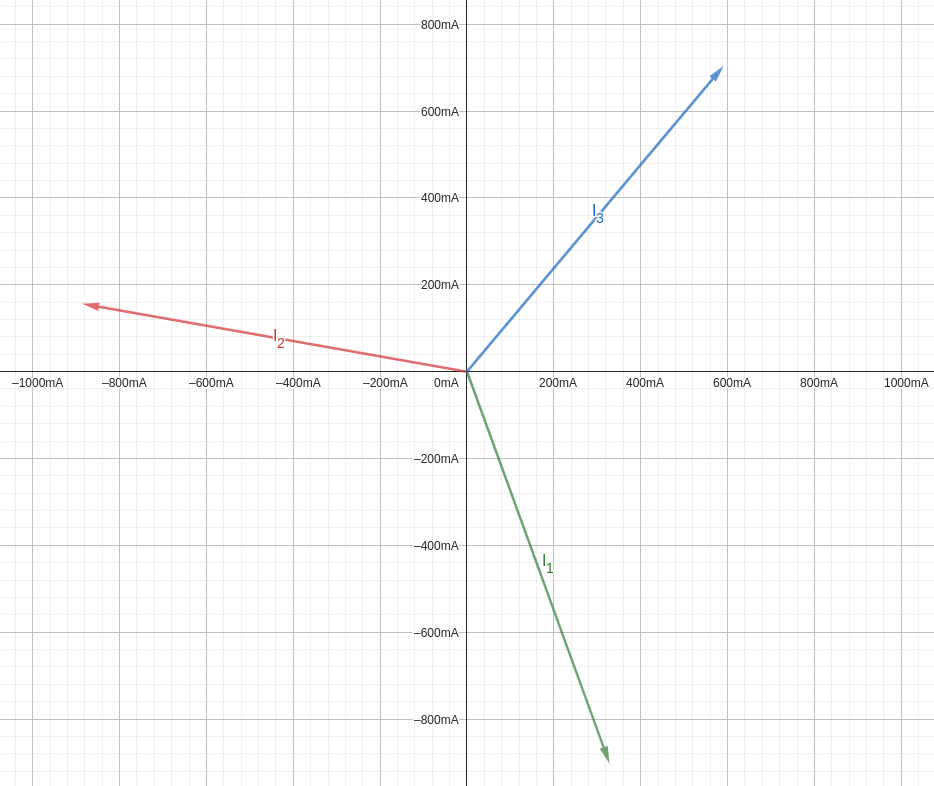
\includegraphics
	 				[width=\textwidth]{img/img3.3.3.png}
	 			\end{subfigure}\hfil
	 			\caption{Skizze der Ströme - Symmetrische Drehstromlast ohne Kompensation}\label{img3.3.3}
	 		\end{figure}
	 				
	 		\newpage
	 		
	 		\item Verbinden Sie nun den Neutralleiter mit dem Knoten K der Sternschaltung und messen Sie den Strom $I_{N}$. Nehmen Sie ein Oszillogramm auf und beschreiben Sie ihre Beobachtungen. Entfernen Sie anschließend wieder die Verbindung zwischen Neutralleiter und Sternpunkt K.
	 		
	 		\begin{figure}[h!]
	 			\centering
	 			\begin{subfigure}[b]{0.7\textwidth}
	 				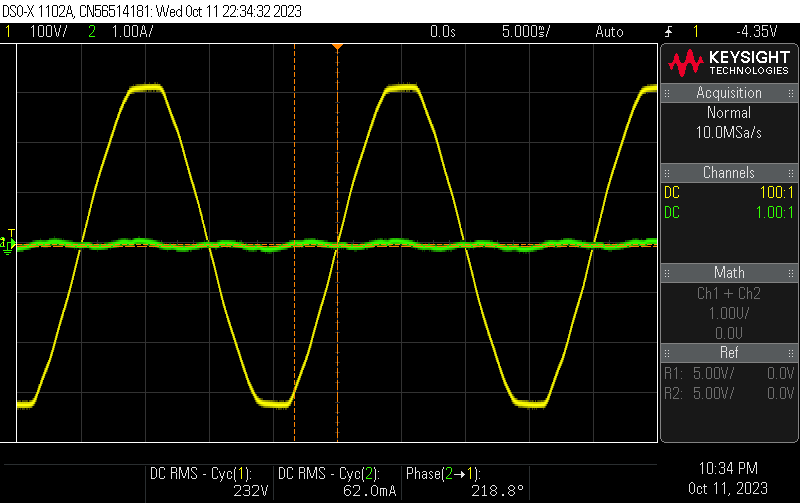
\includegraphics
	 				[width=\textwidth]{img/img3.3.4.png}
	 			\end{subfigure}\hfil
	 			\caption{Oszillogramm von $i_{N}$ - Verbindung zwischen Neutralleiter und Sternpunkt}\label{img3.3.4}
	 		\end{figure}
	 		
	 		\begin{align*}
	 			\underline{I}_{N} &= \underline{I}_{1}+\underline{I}_{2}+\underline{I}_{3} \\
	 			\underline{I}_{N} &= 960\ mA\ e^{-j70^\circ} + 900\ mA\ e^{170^\circ} + 920\ mA\ e^{50^\circ} \\
	 			\underline{I}_{N} &= 52\ mA\ e^{-j50^\circ} \\
 				\Longrightarrow\underline{I}_{N} &\approx 0\ mA
	 		\end{align*}
	 		
	 		
	 		Bei dieser Messung beträgt der Stromfluss im Knotenpunkt zum Neutralleiter ca. $52 mA$. Dieser Strom ist so gering, dass er vernachlässigt werden kann. Alle drei Phasen weisen mehrere komplexe Widerstände auf. Da in allen Phasen derselbe Strom fließt und zwischen ihnen eine Phasenverschiebung von $120^\circ$ besteht, heben sich die Ströme gegenseitig auf, wodurch kein Strom durch den Sternpunkt-Leiter fließt.
	 		
	 		\item Bestimmen Sie aus den Messungen unter (a) die komplexe Impedanz $\underline{Z}_{K}$ in kartesischen Koordinaten durch Mittelung der Werte $\underline{Z}_{1K}$, $\underline{Z}_{2K}$ und $\underline{Z}_{3K}$. Ermitteln Sie anschließend die nötige Kompensationskapazität in Stern- und Dreieckschaltung. Nehmen Sie dazu an, dass die symmetrische Last aus entsprechenden Bauteilen in Reihenschaltung besteht.
	 		
	 		\begin{align*}
	 			\underline{Z}_{K} &= \frac{\underline{U}_{str}}{\underline{I}_{str}}\\
	 			\underline{Z}_{K} &= \frac{U\cdot  e^{j\varphi _{U}}}{I\cdot  e^{j\varphi _{I}}}\\
	 			\underline{Z}_{K} &= \frac{U}{I} \cdot  e^{j\varphi _{U}}\cdot e^{-j\varphi _{I}}\\
	 			\Longrightarrow\underline{Z}_{K} &= \frac{U}{I} \cdot  e^{j{\varphi _{U} - \varphi _{I}}} \\ \ \\
	 			\mid Z \mid			= \frac{U}{I} \hspace{1cm}
	 			\varphi _{Z} 		= {\varphi _{U} - \varphi _{I}}
	 			&\hspace{0.5cm}
	 			Re\{Z\} 			= \mid Z \mid \cdot cos(\varphi _{Z}) \hspace{1cm}
	 			Im\{Z\} 			= \mid Z \mid \cdot sin(\varphi _{Z})\\
	 		\end{align*}
	 		
	 		Um Impedanzen zu bestimmen, wird die Strangspannung durch den Strangstrom geteilt. Die Phase der Strangspannung wird von der Phase des Strangstroms subtrahiert, wodurch die Phasenkomponente der Impedanz ermittelt wird. Impedanzen werden in kartesischer Form ausgedrückt, da aus dieser Form die ohmschen Anteile und die induktiven oder kapazitiven Anteile leicht abgeleitet werden können.
	 		
	 		\begin{center}
	 			\begin{table}[h]
	 				\begin{tabular}{r c c c c c c}
	 					\hline
	 					Art & \( Z\ in\ \Omega\) & \( Phase\ \varphi\ in\ ^\circ\ \ \)  & \( Re{\{z\}} \) & \( Im{\{z\}} \) & \( L\ in\ mH \) & \( C\ in\ \mu H \) \\
	 					\hline
	 					$\underline{Z}_{1K}$ & \( 241 \) & \( 70 \)	& \( 153 \) & \( 187 \) & \( 600 \)	& \( 10,19 \)\\
	 					$\underline{Z}_{2K}$ & \( 260 \) & \( 70 \)	& \( 201 \) & \( 845 \) & \( 640 \)	& \( 9,47 \)\\
	 					$\underline{Z}_{3K}$ & \( 253 \) & \( 70 \)	& \( 160 \) & \( 196 \) & \( 620 \)	& \( 9,73 \)\\
	 					$\underline{Z}_{KN}$ & \( 0   \) & \( 0 \)	& \( 0   \) & \( 0 \)	& \( 0 \)	& \( 0 \)\\
	 					\hline
	 				\end{tabular}
	 				\caption{Messwerte - Komplexe Impedanzen}
	 			\end{table}
	 		\end{center}
	 		
	 		
	 		
	 		\item Beobachten Sie die Spannungen $\underline{u}_{1N}$, $\underline{u}_{2N}$, $\underline{u}_{3N}$ und $\underline{u}_{NK}$ die Ströme $\underline{i}_{1}$, $\underline{i}_{2}$, $\underline{i}_{3}$ und $\underline{i}_{N}$ bei angeschlossener symmetrischer Drehstromlast und drei Kondensatoren $C = 4 \mu F$ in Dreieckschaltung.  Skizzieren Sie die Schaltung und verwenden Sie zur Messung Oszilloskop, Trennteiler und Stromwandler. Halten Sie in einem Satz Ihre Beobachtungen mit einer entsprechenden Begründung fest (ein Oszillogramm in die Ausarbeitung übernehmen und aufarbeiten; $\underline{u}_{1}$ mit $\underline{i}_{1}$).
	 		
	 		\begin{figure}[h!]
	 			\centering
	 			\begin{subfigure}[b]{0.7\textwidth}
	 				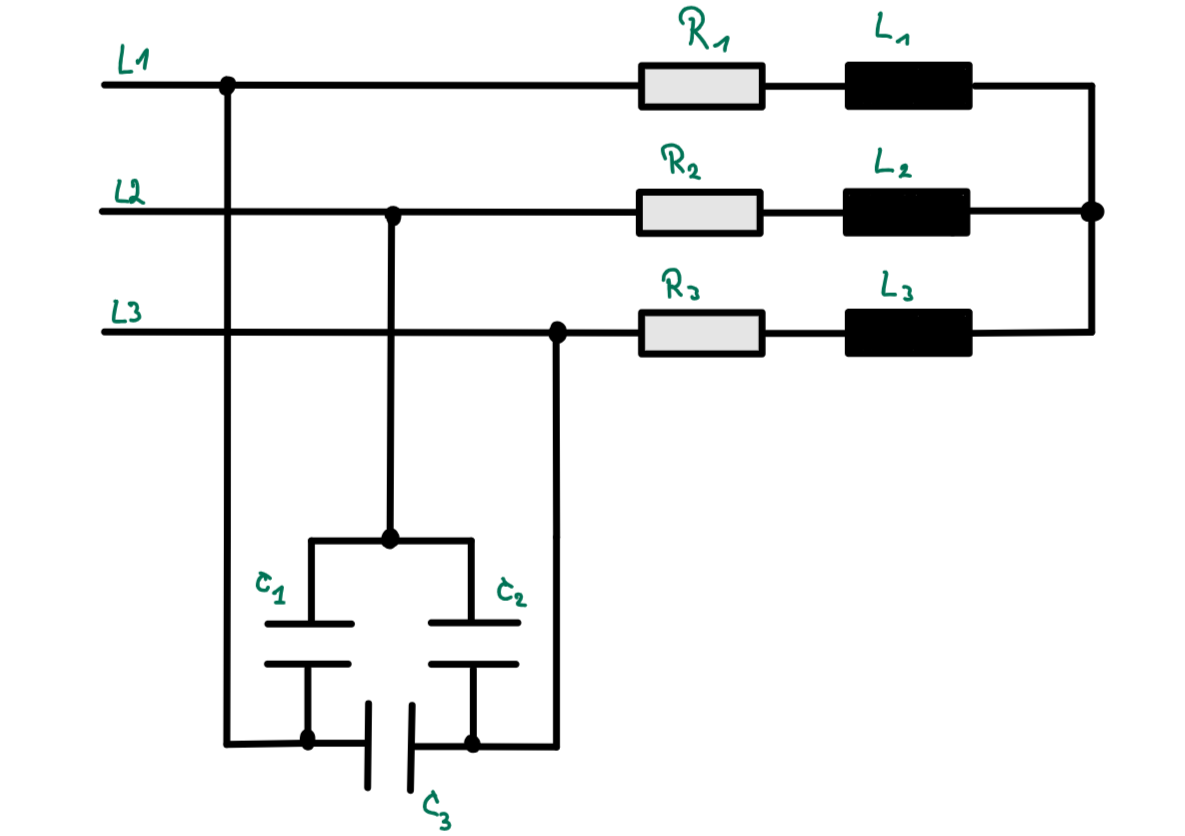
\includegraphics
	 				[width=\textwidth]{img/img3.3.5.png}
	 			\end{subfigure}\hfil
	 			\caption{Skizze zur Kompensation - Symmetrischen Drehstromlast in Dreieckschaltung}\label{img3.3.5}
	 		\end{figure}
	 		
	 		Durch die Implementierung der Kompensation bei der symmetrischen Drehstromlast konnten wir beobachten, dass die zuvor erfolgte Phasenverschiebung zwischen der Spannung $(U)$ und dem Strom $(I)$ vollständig aufgehoben wurde. Dies ist besonders gut auf Abbildung \ref{img3.3.6} zu erkennen, da der Phasenverlauf identisch ist, obwohl der Strom beträchtliche Ober- und Unterschwingungen aufweist. Diese Schwankungen sind eine natürliche Konsequenz der Herstellung von Bauteilen für die symmetrische Drehstromlast, da eine exakte Fertigung nur bis zu einem gewissen Grad möglich ist.
	 		
	 		\begin{figure}[h!]
	 			\centering
	 			\begin{subfigure}[b]{0.7\textwidth}
	 				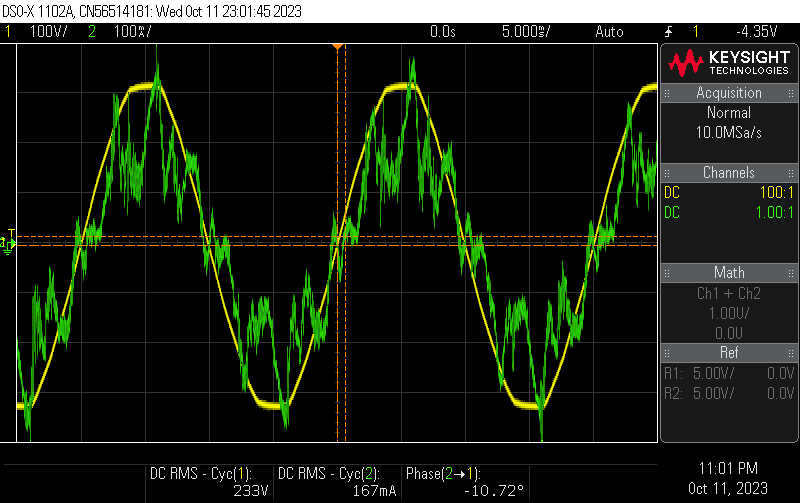
\includegraphics
	 				[width=\textwidth]{img/img3.3.6.png}
	 			\end{subfigure}\hfil
	 			\caption{Oszillogramm von $u_{N}$ und $i_{N}$  - Symmetrischen Drehstromlast in Dreieckschaltung}\label{img3.3.6}
	 		\end{figure}
	 		
	 		
	 		
	 		
	 		\item Schalten Sie nun die drei Kondensatoren in Stern und schließen Sie diese jetzt parallel zur Last an. Überlegen Sie, welche Auswirkungen das auf den Phasenwinkel hat und begründen Sie Ihre Beobachtungen. 
	 		
	 		\begin{figure}[h!]
	 			\centering
	 			\begin{subfigure}[b]{0.7\textwidth}
	 				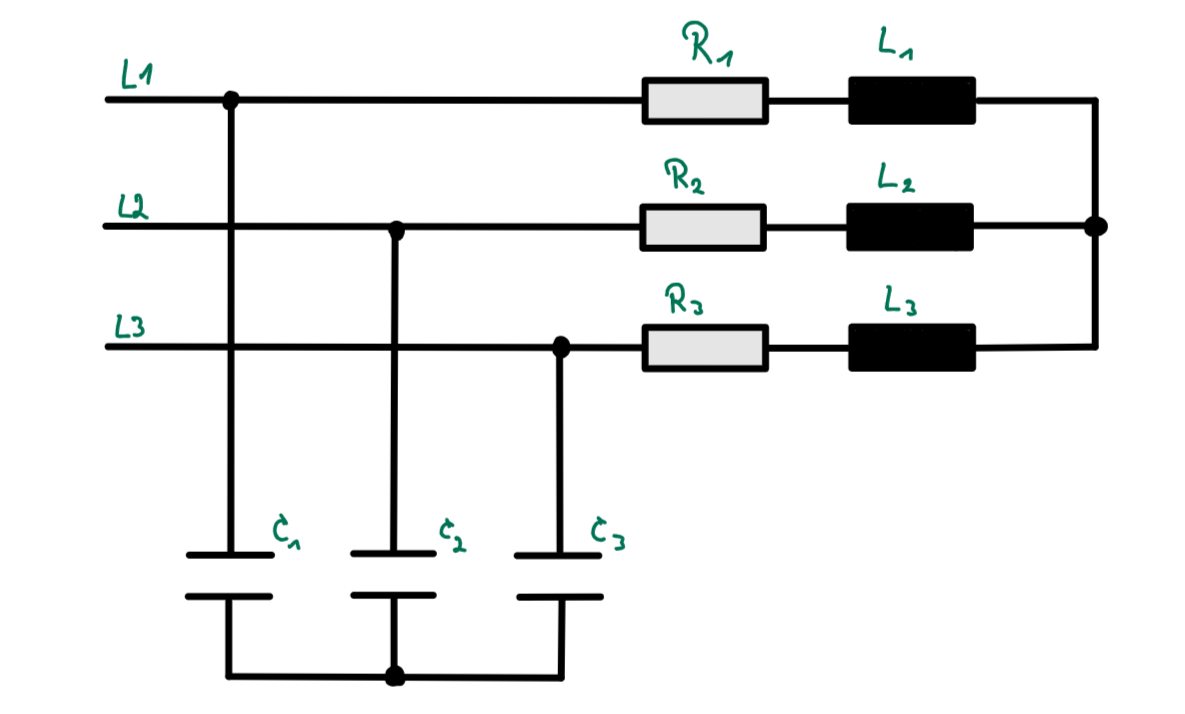
\includegraphics
	 				[width=\textwidth]{img/img3.3.7.png}
	 			\end{subfigure}\hfil
	 			\caption{Skizze zur Kompensation - Symmetrischen Drehstromlast in Sternschaltung}\label{img3.3.7}
	 		\end{figure}
	 		
	 		In Bezug auf die Sternkompensation konnten wir keine Kompensation mit den $4 \mu F$ Kondensatoren feststellen, wie in Abbildung \ref{img3.3.8} dargestellt. Dies liegt daran, dass zwischen der Stern- und Dreieckkompensation ein Faktor von 3 besteht. Um eine Kompensation der Phasenverschiebung zu erreichen, müsste daher ein $12 \mu F$ Kondensator verwendet werden.
	 		
	 		
	 		\begin{figure}[h!]
	 			\centering
	 			\begin{subfigure}[b]{0.7\textwidth}
	 				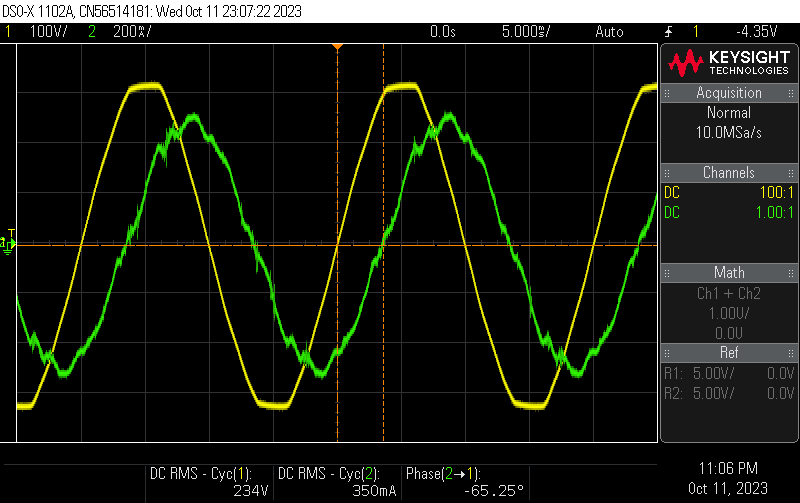
\includegraphics
	 				[width=\textwidth]{img/img3.3.8.png}
	 			\end{subfigure}\hfil
	 			\caption{Oszillogramm von $u_{N}$ und $i_{N}$  - Symmetrischen Drehstromlast in Sternschaltung}\label{img3.3.8}
	 		\end{figure}
	 		
 		\end{enumerate}
 	\subsection{Unsymmetrische Drehstromlast}
	 	\begin{enumerate}[label=\alph*)]
	 		\item Bestimmen Sie die komplexen Effektivwerte der Spannungen $U_{1N}$, $U_{2N}$, $U_{3N}$ und $U_{NK}$ und der Ströme $I_{1}$, $I_{2}$, $I_{3}$ und $I_{K}$ bei der unsymmetrischen Drehstromlast nach Bild 13 \textcolor{red}{mit} angeschlossenem Neutralleiter. (Last je nach Gruppennummer)
	 		\newline
			Skizzieren Sie die Schaltung und verwenden Sie zur Messung Oszilloskop, Trennteiler und Stromwandler. Zwei Oszillogramme sind mit in die Ausarbeitung zu übernehmen und aufzuarbeiten. ($u_{1}$ mit $u_{KN}$, $u_{1}$ mit $i_{N}$).
			
			\item Bestimmen Sie die komplexen Effektivwerte der Spannungen $U_{1N}$, $U_{2N}$, $U_{3N}$ und $U_{NK}$ und der Ströme $I_{1}$, $I_{2}$, $I_{3}$ und $I_{K}$ bei der unsymmetrischen  Drehstromlast nach Bild 13 \textcolor{red}{ohne} angeschlossenem Neutralleiter. (Last je nach Gruppennummer)
			\newline
			Skizzieren Sie die Schaltung und verwenden Sie zur Messung Oszilloskop, Trennteiler und Stromwandler. Zwei Oszillogramme sind mit in die Ausarbeitung zu übernehmen und aufzuarbeiten. ($u_{1}$ mit $u_{KN}$, $u_{1}$ mit $i_{N}$). 
			
			
	 	\end{enumerate}